%!TEX root = ../dissertation.tex
\chapter{Extensive background entropy}
\label{AppendixC}

The imperfect fidelity of the beam splitter operation reduces the interference contrast between the two many-body systems. The measured purities hence underestimate the purity of the many-body states produced in the experiment. 

We verify experimentally that this entropy background contributed by imperfections is extensive. For a separable many-body state, such as a Mott insulator in the atomic limit, we observe an entropy of 0.34 for the full system, or 0.06 per site. 

For the relevant case of superfluid ground states and highly excited quenched states, the measured full system entropy is increased to 0.63. We attribute the loss of the purity in those states tp slight reduction of the beamsplitter contrast for states containing high initial particle numbers (see section~\ref{bs_imperfactions} of the thesis).

We confirm the additive, extensive nature of this background entropy by subtracting the theoretical predicted value of entropy from the measured one as a function of the system size, which shows linear growth of this quantity within our statistics (see Fig.~\ref{fig:ext}). By fitting the data we extract the slope of the curve and apply the correction given by the subsystem size to different plots (see Table 1). With the exception of very short times, these data affirm that the extensive corrections are substantially smaller than the entanglement entropy we measure.

\begin{figure*}
	\centering
	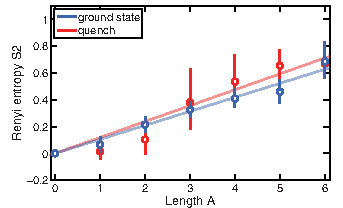
\includegraphics[scale=1.5]{figures/Appendix_extensivity.pdf}
	\caption{The difference between the measured \Renyi entanglement entropy and theoretical calculation as a function of subsystem size. We use the entanglement entropy data of figure~\ref{fig:volume}, averaged over contiguous and non-contiguous sub-systems; the subtracted theory exhibits the same averaging. The linear scaling indicates the presence of an extensive residual entropy background that we attribute to imperfections in the measurement protocol.}
	\label{fig:ext}
	
\end{figure*}

\begin{table*}[t]
	\small
	\begin{center}
		\begin{tabular}{l*{2}{c}}
			\hline
			\\
			& Theory & Data \\
			\hline
			Figure \ref{fig:ETH_purity} & N/A & No Corrections \\
			Figure \ref{fig:EEDyn} & Offset Added & No Corrections \\
			Figure \ref{fig:volume},\ref{fig:MI} & No Corrections & Extensive Entropy Subtracted \\
			\hline
		\end{tabular}
		\caption{\label{tab:Corrections} Listing of all figures that contain data and the numerical corrections applied based upon residual extensive entropy in the system due to beam splitter infidelity.}
	\end{center}
\end{table*}


